\documentclass[12pt]{article}
\usepackage{gensymb}
\usepackage{amssymb}
\usepackage{graphicx}
\begin{document}
\title{Assignment 1 ICSE 2017}
\author{Gunjit Mittal (AI21BTECH11011)}
\maketitle
\section*{Q11 (a)}
The angles of depression of two ships A and B as observed from the top of a light 
house 60 m high are 60\degree and 45\degree
respectively. If the two ships are on the opposite 
sides of the light house, find the distance between the two ships. Give your answer 
correct to the nearest whole number.
\section*{Solution}
\begin{figure}[h]
    \centering
    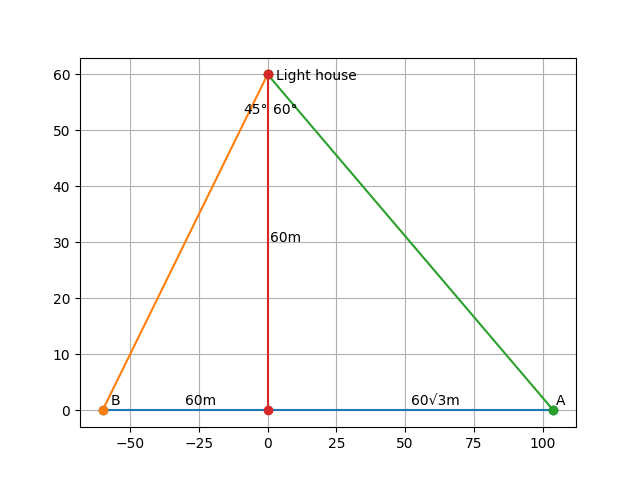
\includegraphics[scale=0.6]{./figs/11.a.png}
\end{figure}
\par 
The distance of ship A from light house is given by $60 \times tan(60\degree) = 60 \times \sqrt{3} $
\newline
The distance of ship B from light house is given by $60 \times tan(45\degree) = 60 $
\newline
Since the two ships are on opposite sides of the light house the distance between them can be obtained by adding their distances to the light house 
\newline
$\therefore$ Distance between ships A and B $= 60 \times \sqrt3 + 60 = 103.92 + 60 = 163.92$
\newline 
$\therefore$ answer $= 164 $

\end{document}
